\section{Simple Linear Regression}
\noindent\rule[\linienAbstand]{\linewidth}{\linienDickeDick}
One of the most important and widely used statistical technique is regression analysis. This is a statistical technique for investigating and modelling relationships between variables.

\subsection{Simple Linear Regression Model}
\noindent\rule[\linienAbstand]{\linewidth}{\linienDicke}
A simple linear regression model is a model with a single predictor variable that has a relationship with a response that is a straight line.\\

\textbf{Model}
\begin{equation}
  y = \beta_0 + \beta_1x \cdot \varepsilon
\end{equation}
where $\beta_0$ and $\beta_1$ are unknown and fixed parameters.\\

\textbf{Variables and error}\\
- Perdictor / input / explanatory variable x (deterministic)\\
- Response / output variable y (random variable)\\
- Uncorrelated random error $\varepsilon $ with
\begin{equation}
  E(\varepsilon ) = 0
\end{equation}
and unknown variance
\begin{equation}
  \textup{Var}(\varepsilon ) = \sigma^2
\end{equation}
Since the error is a random value, y is also a random value.\\

\textbf{Aim}\\
Find Parameters $\hat{\beta}_0, \hat{\beta}_1$ and $\hat{\sigma}^2$ such that model fits data as well as possible.

\textbf{Assumptions}\\
The error $\varepsilon $ is normaly distributed:
\begin{equation}
  E \approx \mathcal{N}(0, \sigma^2) \Rightarrow E(y) = \beta_0 + \beta_1 x
\end{equation}

\subsection{Estimation of the Parameters}
\noindent\rule[\linienAbstand]{\linewidth}{\linienDicke}
\textbf{Method of least square}\\
Minimise:
\begin{equation}
  S(\beta_0, \beta_1) = \sum_{i=1}^n(y_i-(\beta_0 + \beta_1x_i))^2
\end{equation}

Calculating:
\begin{equation}
  \hat{\beta}_0 = \bar{y} - \hat{\beta}_1\bar{x} \;\;\text{with}\;\; \hat{\beta}_1 = \frac{S_{xy}}{S_{xx}}
\end{equation}
where
\begin{equation}
  S_{xx} =  \sum^n_{i=1}(x_i - \bar{x})^2 \;\;\text{and}\;\; S_{xy} =  \sum^n_{i=1}(x_i - \bar{x})(y_i - \bar{y})
\end{equation}
with
\begin{equation}
  \bar{x} = \frac{1}{n}\sum_{i=1}^n x_i  \;\;\text{and}\;\; \bar{y} = \frac{1}{n}\sum_{i=1}^n y_i
\end{equation}

\textbf{Residual}\\
The difference between the $i$th observed value $y_i$ and its fitted value $\hat{y_i}$ is the residual
\begin{equation}
  e_i = y_i - \hat{y}_i = y_i - (\beta_0 + \beta_1x_i)
\end{equation}

\textbf{Mean of residuals}\\
\begin{equation}
  \bar{e} = \frac{1}{n} \sum_{i=1}^n e_i = 0
\end{equation}

\textbf{Unbiased estimator}\\
An unbiased estimator $\hat{\sigma}^2$  is obtained from the error sum of squares
\begin{equation}
  \hat{\sigma}^2 = \frac{1}{n - 2} \sum_{i=1}^n (e_i - \bar{e})^2 = \frac{1}{n - 2} \sum_{i=1}^n e_i^2
\end{equation}
Notice that we have to divide by the degrees of freedom $n - 2$ to make the estimator unbiased. (2 because we have two parameters to find).\\

\textbf{Distribution of the estimators}\\
To be able to answer how well the model fits the data, whether the model can be used as a reliable predictor and whether the the assumptions of constant variance and uncorrelated errors are met, we need to know the distributions of the estimators $\beta_0$ and $\beta_1$.\\
Since the estimators $\beta_0$ and $\beta_1$ are calculated using the random variable $y$, the estimators themselves are random variables which follow the distributions
\begin{equation}
  \hat{\beta}_0 \sim \mathcal{N}\left(\beta_0, \sigma^2\left(\frac{1}{n} + \frac{\bar{x}^2}{S_{xx}}\right)\right)
\end{equation}
and
\begin{equation}
  \hat{\beta}_1 \sim \mathcal{N}\left(\beta_1, \frac{\sigma^2}{S_{xx}}\right).
\end{equation}

\subsection{Tests and Confidence Intervals}
\noindent\rule[\linienAbstand]{\linewidth}{\linienDicke}
In many cases we are not only interested in estimating the model parameters but also in testing hypothesis and constructing confidence intervals.\\

\textbf{Test of a Slope}\\
We use the following hypothesis
\begin{equation}
  \begin{split}
    H_0:& \beta_1 = \beta_{1,0}\\
    H_1:& \beta_1 \neq \beta_{1,0}
  \end{split}
\end{equation}
The null hypothesis states that the observations follow the model of simple linear regression with $\beta_{1} = \beta_{1.0}$ and arbitrary $\beta_0$ and $\sigma$. Where $\beta_{1.0}$ is the slope we want to test.\\

We can estimate the standard error with the error sum of squares.
\begin{equation}
  \textup{se}(\hat{\beta}_1) = \sqrt{\frac{\hat{\sigma}^2}{S_{xx}}} \text{    with    } S_{xx} =  \sum^n_{i=1}(x_i - \bar{x})^2
\end{equation}

The test statistic is the following
\begin{equation}
  T = \frac{\hat{\beta}_1 - \beta_{1,0}}{\textup{se}(\hat{\beta}_1)}
  \label{eq:7.3.b}
\end{equation}
Under the null hypothesis the test statistic $T$ follows a Student’s t-distribution with $n - 2$ degrees of freedom. Values of t are usually found in a table.\\
If T is smaller than t (from the table), we accept the null hypothesis and conclude that the data agrees also with a model with the slope $\beta_{1,0}$.\\


The \textbf{P-Value} is the probability, under the null hypothesis, of obtaining a result equal to or more extreme than what was actually estimated. If the value T of the test statistic is larger than the critival value t (from the table) the null hypothesis is not rejected i.e. it is plausible to assume that the data fits the model.\\

The test statistic \ref{eq:7.3.b} is accepted on the significance level $\alpha$ if
\begin{equation}
  t_{\frac{\alpha}{2}, n-2} \leq T \leq t_{-\frac{\alpha}{2}, n-2},
\end{equation}
which leads us to the following \textbf{confidence interval on the slope}
\begin{equation}
  \hat{\beta}_1 - t_{\frac{\alpha}{2}, n-2} \cdot \textup{se}(\beta_1)
  \leq \beta_1 \leq
  \hat{\beta}_1 + t_{-\frac{\alpha}{2}, n-2} \cdot \textup{se}(\beta_1)
\end{equation}
\begin{equation}
  \left[
  \hat{\beta}_1 - t_{\frac{\alpha}{2}, n-2} \cdot \textup{se}(\beta_1),
  \hat{\beta}_1 - t_{-\frac{\alpha}{2}, n-2} \cdot \textup{se}(\beta_1)\right].
\end{equation}
Interpretation: The true value of $\beta_1$ lies in the confidence interval with high probability.

\subsection{Confidence Interval of the Response}
\noindent\rule[\linienAbstand]{\linewidth}{\linienDicke}
The estimated response of a regression model is as follows:
\begin{equation}
  \hat{y}_0 = \hat{\beta}_0 +  \hat{\beta}_1 x_0
\end{equation}

Now we want to find a confidence interval on the response. Such a confidence interval corresponds to the null hypothesis
\begin{equation}
  H_0: \hat{y}_0 = \mu_0
\end{equation}

The estimator $\hat{y}_0$ is normally distributed, unbiased and has the variance
\begin{equation}
  \textup{Var}(\hat{y}_0) = \sigma^2\left(\frac{1}{n} + \frac{(x_0 - \bar{x})^2}{S_{xx}}\right)
\end{equation}

As usual $\sigma^2$ is in general unknown and has to be estimated from the data. The test statistic about the response is
\begin{equation}
  T = \frac{\hat{y}_0 - \mu_0}{\textup{se}(\hat{y}_0)}.
\end{equation}
with the standard error
\begin{equation}
  \textup{se}(\hat{y}_0)=\hat{\sigma}\sqrt{\frac{1}{n} + \frac{(x_0 - \bar{x})^2}{S_{xx}}}
\end{equation}
Under the null hypothesis the test statistic $T$ follows a Student’s $t$-distribution with $n - 2$ degrees of freedom.\\
The \textbf{confidence interval} on the response at the point $x_0$ is
\begin{equation}
  \hat{y}_0 - t_{\frac{\alpha}{2},n-2} \cdot \textup{se}(\hat{y}_0)
  \leq \mu_0 \leq
  \hat{y}_0 + t_{1 - \frac{\alpha}{2},n-2} \cdot \textup{se}(\hat{y}_0)
\end{equation}

\subsection{Prediction Interval}
\noindent\rule[\linienAbstand]{\linewidth}{\linienDicke}
The point estimate of a new value of the response $y_0$ is
\begin{equation}
  \hat{y}_0 = \hat{\beta}_0 +  \hat{\beta}_1 x_0.
\end{equation}
Now our aim is to find a prediction interval for a future observation. It is very important to understand that in this situation the randomness of the future observation $y_0$ has to be considered too. Therefore the random variable $y_0 - \hat{y}_0$ has to be considered.\\
To calculate its variance we use the formula for the difference of two uncorrelated random variables
\begin{equation}
  \textup{Var}(X - Y) = \textup{Var}(X) + \textup{Var}(Y)
\end{equation}
Therefore
\begin{equation}
  \begin{split}
      \textup{Var}(y_0 - \hat{y}_0) &= \textup{Var}(y_0) + \textup{Var}(\hat{y}_0)\\
      &= \sigma^2\left(1 + \frac{1}{n} + \frac{(x_0 - \bar{x})^2}{S_{xx}}\right)
  \end{split}
\end{equation}
The prediction interval is wider than the confidence interval on the response, since the variance of the future observation has to be considered too. As usual $\sigma^2$ is in general unknown and has to be estimated from the data.

The \textbf{prediction interval} at the point $x_0$ is
\begin{equation}
  \hat{y}_0 - t_{\frac{\alpha}{2},n-2} \cdot \textup{se}(y_0 - \hat{y}_0)
  \leq \hat{y}_0 \leq
  \hat{y}_0 + t_{1 - \frac{\alpha}{2},n-2} \cdot \textup{se}(y_0 - \hat{y}_0)
\end{equation}
with
\begin{equation}
  \textup{se}(y_0 - \hat{y}_0) = \hat{\sigma}\sqrt{1 + \frac{1}{n} + \frac{(x_0 - \bar{x})^2}{S_{xx}}}
\end{equation}

\begin{figure}[H]
  \centering
  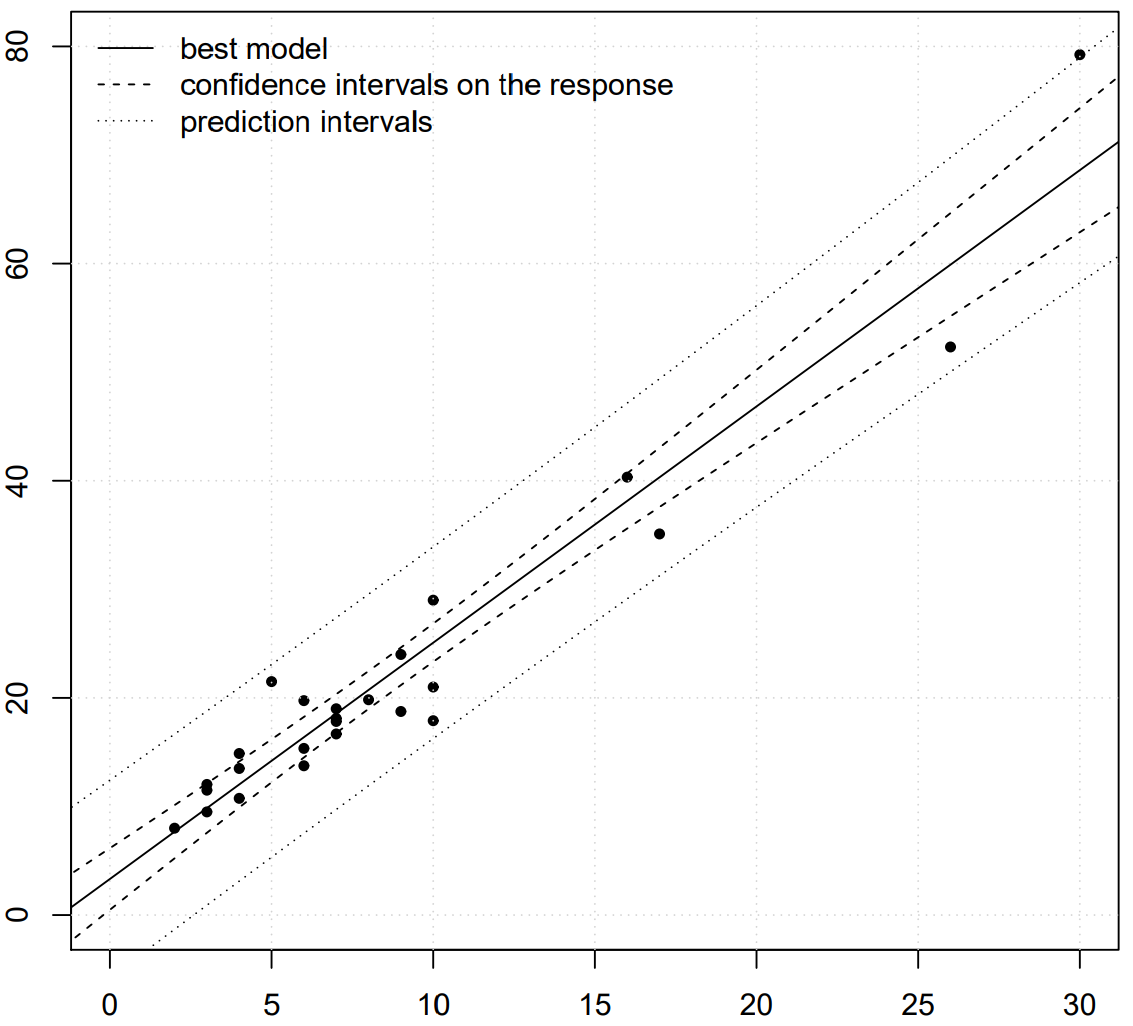
\includegraphics[width=0.8\linewidth]{Pics/7.4.png}
\end{figure}
